\documentclass[a4paper,12pt]{article}
\usepackage[utf8]{ inputenc}
\usepackage[ngerman]{babel}
\usepackage[a4paper, left=2.5cm, right=2.5cm]{geometry}
\usepackage{graphicx}
\usepackage{subcaption}
\usepackage{fancyhdr}
\usepackage{pdfpages}
\usepackage{listings}
\usepackage{hyperref}
\usepackage[official]{eurosym}
\usepackage{float}

\pagestyle{fancy}
\lstset{
	language=Matlab,
	breaklines=true,
	morekeywords={matlab2tikz},
	keywordstyle=\color{blue},
	morekeywords=[2]{1}, keywordstyle=[2]{\color{black}},
	identifierstyle=\color{black},
	stringstyle=\color{mylilas},
	commentstyle=\color{mygreen},
	showstringspaces=false,
	mathescape=true
	emph=[1]{for,end,break},emphstyle=[1]\color{red},
}

\lhead{Investitionsrechnung für Haushalte}
\chead{}
\rhead{Gruppe D}

\begin{document}
	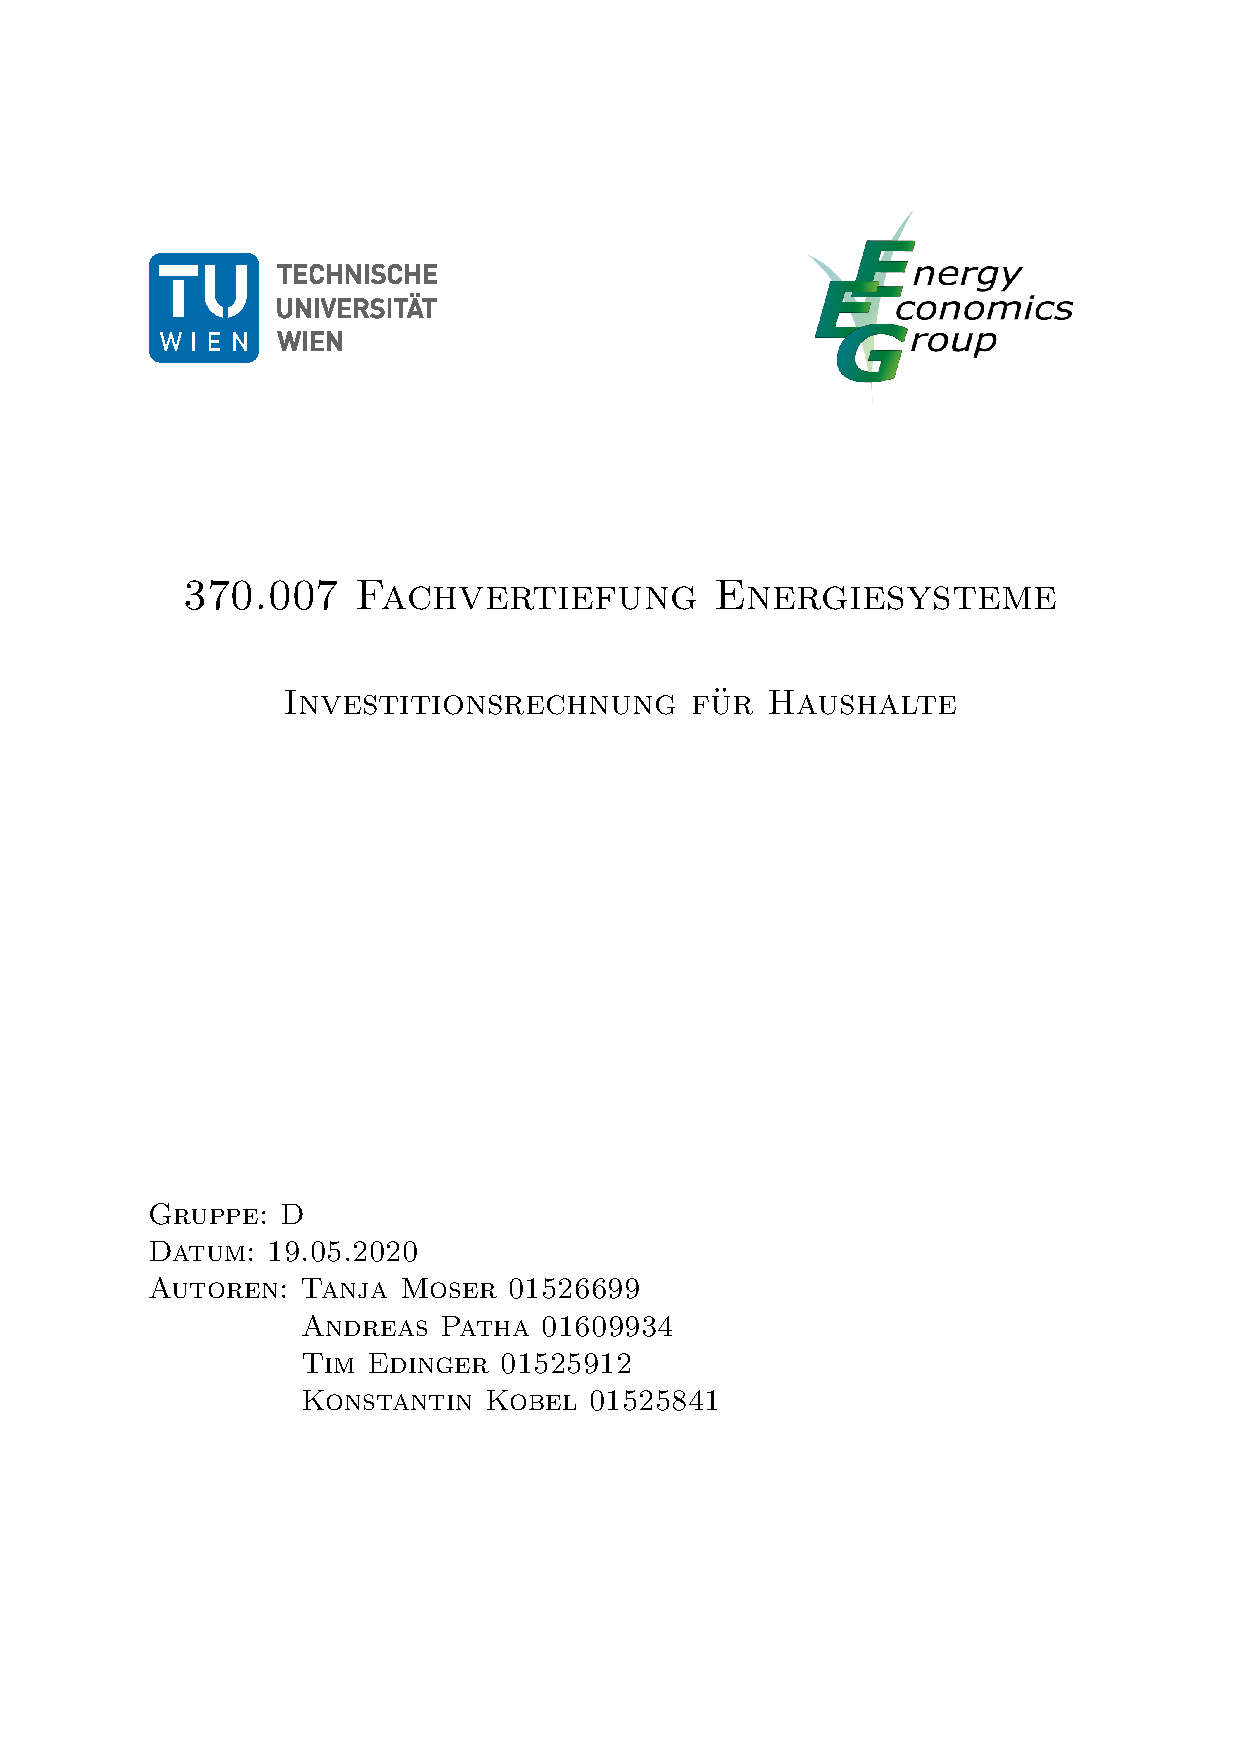
\includepdf{Protokoll_titlepage.pdf}

	\newpage
	\tableofcontents

	\newpage
	\section{Aufgabenstellung}
	\label{sec:Aufgabenstellung}
	Das Ziel der dritten Übung ist es, die Wirtschaftlichkeit einer PV-Anlage, für einen Haushalt, zu errechnen.\newline
	Die Wirtschaftlichkeitsrechnung ist ein wichtiges Instrument um Technologien aus volkswirtschaftlicher Sicht zu bewerten,
	Unternehmen eine Hilfe bei Investitionsentscheidungen zu bieten, staatliche Förderungen zu planen und Zahlungen an unterschiedlichen Zeitpunkten zu bewerten.
	\subsection{Aufgabe 3.1}
	\label{sec:Aufgabenstellung31}
	Aufgabe 3.1 befasst sich mit dem Barwert (= dem Kapitalwert) einer $10kWp$ PV-Anlage.\newline
	In dieser ersten Aufgabe wird davon ausgegangen, dass die gesamte Produktion verkauft wird.\\ \par
	\noindent Zur Berechnung werden folgende \textbf{Parameter} definiert:
	\begin{itemize}
		\item Der Zinssatz beträgt $4\%$.
		\item Die Systemkosten betragen $1200\mbox{\euro}/kWp$.
		\item Die Betriebskosten/die Versicherung belaufen sich auf $4\mbox{\euro}/(kWp\,a)$.
		\item Die Lebensdauer der PV-Anlage kann mit $25$ Jahren angenommen werden.
		\item Der $Einspeisetarif_{OeMAG}$ beträgt $8.24\,Cent/kWh$.
		\item Die $F\ddot{o}rderdauer_{OeMAG}$ beträgt $13$ Jahre.
		\item Die relevanten Spotpreise werden in der Datei $Spotpreise.mat$ zur Verfügung gestellt.
		\item Informationen zu Förderungen können folgendem Link entnommen werden:\newline
		\url{http://www.oem-ag.at/de/foerderung/photovoltaik/}
	\end{itemize}
	Es werden folgende \textbf{Annahmen} getroffen:
	\begin{itemize}
		\item Das Jahr 2016 steht exemplarisch für jedes kommende Jahr.
		\item Auch nach dem Vertragsende wird der Strom, bis zum Ende der Lebensdauer, am Spotmarkt verkauft. Die Preise entsprechen dabei den Preisen aus dem Jahr 2016.
	\end{itemize}
	Die \textbf{Aufgaben} lauten:
	\begin{itemize}
		\item[a)] Berechnen Sie den Barwert (= Kapitalwert) einer 10 kWp PV-Anlage unter der Annahme, dass die gesamte Produktion am Spotmarkt verkauft wird.
		\begin{itemize}
			\item Wie hoch dürfen die Investitionskosten maximal sein, damit die Wirtschaftlichkeit der Investition positiv bewertet wird (Barwert > 0)?
			\item Stellen Sie die Entwicklung des Kapitalwerts (=Barwert) der Investition über die Lebensdauer in einem Diagramm dar.
		\end{itemize}
		\item[b)] Führen Sie die Berechnung noch einmal unter der Annahme durch, dass Sie den aktuellen OeMAG Einspeisetarif für 13 Jahre erhalten.\newline Vergleich Sie diesen Fall mit dem nicht geförderten Fall.
	\end{itemize}
	\subsection{Aufgabe 3.2}
	\label{sec:Aufgabenstellung32}
	In Aufgabe 3.2 wird der Eigenverbrauch der Haushalte berücksichtigt und nur noch der Überschuss der Produktion verkauft.\\ \par
	\noindent Folgende \textbf{Parameter} sind gegeben:
	\begin{itemize}
		\item Es handelt sich um eine $5kWp$ PV-Anlage.
		\item Das Einspeiseprofil der PV-Anlage wird in der Datei $PV_Einspeiseprofil.mat$ zur Verfügung gestellt.
		\item Der Standort der PV-Anlage ist Wien.
		\item Die Ausrichtung der PV-Anlage ist mit einem Azimut von $180^{\circ}$ und einem Neigungswinkel von $30^{\circ}$ gegeben.
		\item Die benötigte Leistung der Haushalte ist in der Datei $LeistungHaushalte.mat$ definiert.
	\end{itemize}
	Die \textbf{Aufgaben} lauten:
	\begin{itemize}
		\item[a)] Berechnen Sie den Eigenverbrauch und die Überschusseinspeisung einer $5kWp$-Anlage für 5 der gegebenen 30 Haushalte.
		\item[b)] Stellen Sie die Entwicklung des Eigenverbrauchsanteils und der Deckungsgrade der Haushalte für eine Anlagengröße von $0kWp$ bis $20kWp$ für die 5 Haushalte dar.
		\item[c)] Erstellen Sie eine Grafik, in der die Erzeugung, die Last und der Eigenverbrauch für die Woche 3 und 25 für Haushalt 1 dargestellt wird. Verwenden Sie für die Darstellung des Eigenverbrauchs die Plot-Funktion $area$.
	\end{itemize}
	\subsection{Aufgabe 3.3}
	In Aufgabe 3.3 sollen die Berechnungen von Aufgabe 3.2 erweitert werden.\\ \par
	\noindent Dazu werden folgende \textbf{Annahmen} getroffen:
	\begin{itemize}
		\item Für den Eigenverbrauch kann eine Ersparnis in Höhe des Haushaltsstrompreises angesetzt werden. Diese beträgt $15\,Cent/kWh$.
		\item Für die Überschusseinspeisung kann ein Einspeisetarif von $5\,Cent/kWh$ angenommen werden.
	\end{itemize}
	Die \textbf{Aufgaben} lauten:
	\begin{itemize}
		\item[a)] Erstellen Sie eine Investitionsrechnung (Barwert) für die 5 gegebenen Haushalte und einer Anlagengröße von $5kWp$. Vergleichen Sie dazu den Fall mit PV-Anlage mit dem Fall ohne PV-Erzeugung.
		\item[b)] Wie hoch dürfen die spezifischen Investitionskosten (EUR/kW) je Haushalt maximal sein, damit die Investition als wirtschaftlich gewertet wird?
	\end{itemize}
	\subsection{Aufgabe 3.4}
	In Aufgabe 3.4 soll eine Beurteilung von PV-Anlagen in Österreich, auf Basis der in den vorigen Aufgaben durchgeführten Berechnungen, getroffen werden.\\ \par
	\noindent Die \textbf{Fragen} lauten:
	\begin{itemize}
		\item[a)] Erstellen Sie eine Investitionsrechnung (Barwert) für die 5 gegebenen Haushalte und einer Anlagengröße von $5kWp$. Vergleichen Sie dazu den Fall mit PV-Anlage mit dem Fall ohne PV-Erzeugung.
		\item[b)] Wie hoch dürfen die spezifischen Investitionskosten (EUR/kW) je Haushalt maximal sein, damit die Investition als wirtschaftlich gewertet wird?
	\end{itemize}
	\newpage
	\section{Berechnungen}
	\label{sec:Berechnungen}
	\subsection{Zinsen}
	Wie bereits im Kapitel \hyperref[sec:Aufgabenstellung]{Aufgabenstellung} erwähnt, ist die Wirtschaftlichkeitsrechnung ein wichtiges Instrument für unterschiedlichste Akteure.\newline
	Einen starken Einfluss auf diese Berechnung haben Zinsen.\\ \par
	\noindent Zinsen bezeichnen in der Wirtschaft das Entgelt, das der Schuldner dem Gläubiger als Gegenleistung für vorübergehend überlassenes Kapital zahlt.\\ \par
	\noindent Sie haben mehrere Interpretationen und Funktionen:
	\begin{itemize}
		\item Funktion des \textbf{Entgelts für entliehenes Kapital}. In diesem Fall geht es um einen Mindest-Zinssatz der erreicht werden muss um die minimalen Kosten des Kapitaleinsatzes zu decken.
		\item Funktion der \textbf{Zeitpräferenz}. Sie beschreibt die Präferenz den Konsum in der Gegenwart zu tätigen und nicht auf einen zukünftigen Zeitpunkt zu warten.
		\item Funktion des \textbf{Allokationsmechanismus}. Diese Interpretation erlaubt Messungen und bietet eine Entscheidungshilfe. Die Funktion der Zinsen ist in diesem Fall, dass das "knappe Gut" Kapital möglichst sinnvoll verteilt wird.
		\item Funktion des \textbf{Risikoindikators}. Das mit der Investition verbundene Risiko hat einen starken Einfluss auf den Zinssatz.
	\end{itemize}
	Die Zahlungsströme (= Cash Flows) werden durch Zinsen gewichtet.
	\subsubsection{Aufzinsen}
	Beim Aufzinsen geht es um die Frage nach dem Wert von Kapital, nach $n$ Jahren. Für die Berechnung gehen wir davon aus, dass das Kapital zum Zeitpunkt $t=0$ eingezahlt wird.\\ \par
	\noindent Die Berechnung kann mit folgender Formel erfolgen:
	\begin{equation}
	K_n=K_0*(1+r)^n
	\end{equation}
	\begin{itemize}
		\item $K_n$ entspricht dem Wert des Kapitals nach $n$ Jahren.
		\item $K_0$ ist der Wert des Kapitals zum Zeitpunkt der Einzahlung. (zum Zeitpunkt $t=0$)
		\item $n$ ist die Dauer des Betrachtungszeitraums in Jahren.
		\item $r$ entspricht dem Zinssatz pro Jahr.
	\end{itemize}
	Der Wert des Kapitals wächst bei einem positiven Zinssatz $r$ nach $n$ Perioden exponentiell an.
	\subsubsection{Abzinsen}
	Bei der Bewertung einer Investition wird üblicherweise der Wert des zukünftigen Zahlungsstroms, zum Zeitpunkt $t=0$, ermittelt. Dieser Wert wird dann der Investition gegenübergestellt.\\ \par
	Die Berechnung kann mit Hilfe folgender Formel durchgeführt werden:
	\begin{equation}
	K_0=\frac{K_n}{(1+r)^n}
	\end{equation}
	\begin{itemize}
		\item $K_n$ ist der Wert des Kapitals nach $n$ Jahren.
		\item $K_0$ entspricht dem Wert des Kapitals zum Zeitpunkt der Einzahlung. (zum Zeitpunkt $t=0$)
		\item $n$ ist die Dauer des Betrachtungszeitraums in Jahren.
		\item $r$ entspricht dem Zinssatz pro Jahr.
	\end{itemize}
	\subsection{Barwertmethode}
	\label{sec:BerechnungenBarwertmethode}
	Die Barwertmethode ist eine Methode der dynamischen Wirtschaftlichkeitsberechnung bei der der Barwert (= Net Present Value $NPV$) errechnet wird. Sie liefert eine Aussage über die Sinnhaftigkeit einer Investition.\\ \par
	\noindent Zur Bestimmung des Barwertes einer Investition werden alle Zahlungsströme (= Cash Flows), eines bestimmten Betrachtungszeitraumes, auf den Zeitpunkt $t=0$, mit dem erwarteten Zinssatz $r$, abgezinst und addiert. Damit werden alle Zahlungen auf den Zeitpunkt $0$ bezogen.\\ \par
	\noindent Die Berechnung des Net Present Values erfolgt mit folgender Formel:
	\begin{equation}
	NPV=-I_0+\frac{E_1-A_1}{(1+r)}+\frac{E_2-A_2}{(1+r)^2}+...+\frac{E_n-A_n}{(1+r)^n}+\frac{L}{(1+r)^n}
	\end{equation}
	Andere Schreibweisen dieser Formel sind
	\begin{equation}
	NPV=-I_0+\frac{CF_1}{(1+r)}+\frac{CF_2}{(1+r)^2}+...+\frac{CF_n}{(1+r)^n}+\frac{L}{(1+r)^n}
	\end{equation}
	oder
	\begin{equation}
	NPV=-I_0+\sum_{i=1}^n\frac{CF_i}{(1+r)^i}+\frac{L}{(1+r)^n}
	\end{equation}
	\begin{itemize}
		\item $NPV$ entspricht dem Nettobarwert der Investition in Euro.
		\item $I_0$ sind die Investitionskosten zum Zeitpunkt $0$ in Euro.
		\item $E_i$ sind die Einnahmen in der Periode $i$ in Euro.
		\item $A_i$ sind die Ausgaben und Kosten in der Periode $i$ in Euro.
		\item $CF_i$ entspricht dem Cash Flow in der Periode $i$ in Euro. ($E_i-A_i$ entspricht einem Cash Flow)
		\item $r$ ist der gewählte Kalkulationszinssatz bei der Barwertrechnung bzw. der gesuchte Zinssatz bei der Berechnung des internen Zinsfuß.
		\item $L$ ist der Restwert der Investition am Ende des Betrachtungszeitraums in Euro.
		\item $n$ entspricht der Dauer des Betrachtungszeitraums in Jahren.
	\end{itemize}
	Wie bereits eingangs beschrieben, trifft die Barwertmethode eine Aussage über die Sinnhaftigkeit einer Investition.\newline Wenn der Wert $NPV$ größer als $0$ ist, lohnt sich die Investition. Ist der $NPV$ kleiner als $0$, sollte von einer Investition abgesehen werden.
	\subsection{Eigenverbrauch und Überschusseinspeisung}
	\label{sec:eigenverbrauchueberschusseinspeisung}
	Bei den Berechnungen zum Eigenverbrauch und der Überschusseinspeisung wird von einem oder mehreren Haushalten, mit eigener Strom Produktion, ausgegangen.\\ \par
	In diesem Kontext sind drei Begriffe relevant:
	\begin{itemize}
		\item \textbf{Eigenverbrauchsanteil} - Der Eigenverbrauchsanteil entspricht dem Anteil des Eigenverbrauchs an der eigenen Gesamterzeugung.\\ \par
		\noindent Die Berechnung erfolgt über die Formel
		\begin{equation}
		Eigenverbrauchsanteil=\frac{Eigenverbrauch}{Gesamterzeugung}
		\end{equation}
		\item \textbf{Deckungsgrad} - Der Deckungsgrad ist das Verhältnis des Eigenverbrauchs zum gesamten Stromverbrauch.
		Er gibt den Anteil des Stromverbrauchs an, der durch die eigene Produktion gedeckt werden kann.\\ \par
		\noindent Die Formel, zur Berechnung, lautet
		\begin{equation}
		Deckungsgrad=\frac{Eigenverbrauch}{Stromverbrauch}
		\end{equation}
		\item \textbf{Energetischer Deckungsgrad} - Der energetische Deckungsgrad gibt das Verhältnis der Gesamterzeugung zum gesamten Stromverbrauch an.\\ \par
		\noindent Die Formel lautet
		\begin{equation}
		Deckungsgrad_{energetisch}=\frac{Gesamterzeugung}{Stromverbrauch}
		\end{equation}
	\end{itemize}
	\newpage
	\section{Ergebnisse}
	\subsection{Aufgabe 3.1 -Verkauf der gesamten Produktion}
	\subsubsection{3.1.a - Barwert einer 10kWp PV-Anlage bei Verkauf am Spotmarkt}
	In Aufgabe 3.1.a soll der Barwert einer $10kWp$ Anlage berechnet werden. Im ersten Fall wird davon ausgegangen, dass die gesamte Produktion der PV-Anlage am Spotmarkt verkauft wird. Die Parameter der PV-Anlage, sowie die Spotmarktpreise, können Kapitel \hyperref[sec:Aufgabenstellung31]{Aufgabe 3.1} entnommen werden.\newline
	Die Vorgangsweise, zur Ermittlung des Barwertes, wird in Kapitel \hyperref[sec:BerechnungenBarwertmethode]{Barwertmethode} erklärt.\\ \par
	\noindent Da die Datei $Spotpreis.mat$ die stündlichen Preise für nur neun Jahre beinhaltet, werden die Preise des neunten Jahres für die restlichen 16 Jahre des Betrachtungszeitraums genommen.\newline In MATLAB ergibt sich dadurch folgender Code:
	\begin{lstlisting}
	NPV=$-$Systemkosten*Anlagenleistung;

	Investitionszuschuss = min(Systemkosten*Anlagenleistung*Investitionszuschuss_prozent, Investitionszuschuss_max*Anlagenleistung);
	
	for i = 1:25
		if i <= 9
			Preis_i=table2array(Spotpreis(:,i))./100;
		else
			Preis_i=table2array(Spotpreis(:,9))./100;
		end
		CF=sum(PV_profil.*Anlagenleistung.*Preis_i)+Investitionszuschuss$-$Betriebskosten*Anlagenleistung;
	
		NPV=NPV+CF/(1+Zinssatz)^i;
	end
	\end{lstlisting}
	\begin{itemize}
		\item \textbf{NPV} ist der Net Present Value der PV-Anlage, für das jeweilige Jahr.
		\item \textbf{Investitionszuschuss} entspricht dem jährlichen Investitionszuschuss.
		\item \textbf{CF} entspricht der Summe der Cash Flows, für das jeweilige Jahr.
		\item \textbf{Anlagenleistung} entspricht einem Wert von $10$ (in $kWp$).
		\item \textbf{Zinssatz} ist $0.04$ (in \%).
		\item \textbf{Systemkosten} beträgt $1200$ (in $\mbox{\euro}/kWp$).
		\item \textbf{Betriebskosten} entspricht $4$ (in $\mbox{\euro}/kWp$).
	\end{itemize}
	Der Verlauf des NPV, der Anlage, wird in der oberen Hälft von Abbildung 1 dargestellt.\\ \par
	\noindent Zusätzlich sollten die maximalen Investitionskosten ermittelt werden, damit die Wirtschaftlichkeit der Investition positiv bewertet wird. Diese errechnen sich aus dem NPV nach 25 Jahren plus der Investitionskosten.
	\begin{lstlisting}
	Max_Invest_Gesamtverkauf = NPV + Anlagenleistung*Systemkosten;
	\end{lstlisting}
	Die maximalen Investitionskosten für die positive Bewertung der Wirtschaftlichkeit, im Fall, dass die gesamte Produktion am Spotmarkt verkauft wird, sind $50.964\mbox{\euro}$.
	\subsubsection{3.1.b - Barwert einer 10kWp PV-Anlage mit Förderung}
	In Aufgabe 3.1.b soll die Berechnung von Aufgabe 3.1.a dahingehend erweitert werden, dass man eine Förderung in der Höhe des aktuellen OeMAG Einspeisetarif für 13 Jahre erhält. Nach Vertragsende wird der Strom bis zum Ende der Lebensdauer am Spotmarkt verkauft.\newline
	Der MATLAB Code aus Aufgabe 3.1.a muss für die neue Annahme folgendermaßen erweitert werden:
	\begin{lstlisting}
	NPV = $-$Systemkosten*Anlagenleistung;
	
	for i = 1:25
		if i <= Foerderdauer
			Preis_i = Einspeisetarif;
		else
			Preis_i = table2array(Spotpreis(:,9))./100;
		end
		CF = sum(PV_profil.*Anlagenleistung.*Preis_i)+Investitionszuschuss$-$ Betriebskosten*Anlagenleistung;

		NPV = NPV + CF/(1+Zinssatz)^i;
	end
	\end{lstlisting}
	\begin{itemize}
		\item \textbf{Einspeisetarif} entspricht $0.0824$ (in $\mbox{\euro}$).
		\item \textbf{Foerderdauer} ist $13$ (in Jahren).
	\end{itemize}
	Das Ergebnis für Aufgabe 3.1.b wird in der unteren Hälfte von Abbildung 1 dargestellt.
	\subsubsection{Vergleich von Aufgabe 3.1.a und Aufgabe 3.1.b}
	\begin{figure}[H]
		\centering
		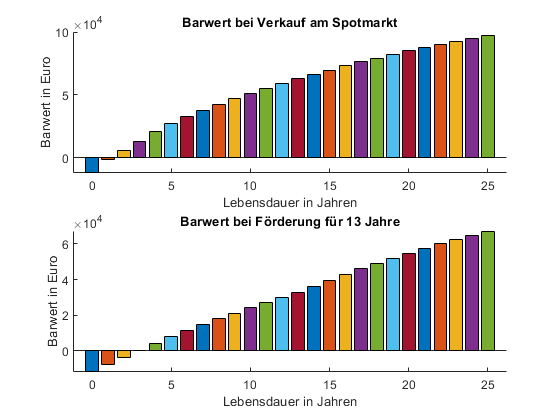
\includegraphics[width=12cm]{img/results/BarwertVergleich}
		\caption{Der Barwert, der in Kapitel Aufgabe 3.1 definierten PV-Anlage, über einen Betrachtungszeitraum von 25 Jahren.}
	\end{figure}
	Wie bereits in Kapitel \hyperref[sec:BerechnungenBarwertmethode]{Barwertmethode} erwähnt, trifft die Barwertmethode eine Aussage über die Sinnhaftigkeit einer Investition.\newline
	Der Vergleich in Abbildung 1 zeigt, dass der Barwert der PV-Anlage im Fall aus Aufgabe 3.1.a bereits im zweiten Jahr positiv ist. (ein positiver NPV spricht für die Investition, ein negativer dagegen)\newline
	Unter der Annahme aus Aufgabe 3.1.b erreicht die PV-Anlage nach vier Jahren einen positiven NPV. Weiters ist der NPV, aus Aufgabe 3.1.a, nach 25 Jahren bei ungefähr $100.000\mbox{\euro}$, während der NPV aus Aufgabe 3.1.b nach 25 Jahren nur circa $60.000\mbox{\euro}$ beträgt.\newline
	Demnach ist der Verkauf der gesamten Produktion auf dem Spotmarkt lukrativer, als die Förderung der PV-Anlage.
	\subsection{Aufgabe 3.2 - Eigenverbrauch}
	\subsubsection{Aufgabe 3.2.a - Eigenverbrauch und Überschusseinspeisung}
	In Aufgabe 3.2.a soll der Eigenverbrauch und die Überschüsseinspeisung einer $5kWp$ Anlage, mit Standort Wien, für 5 Haushalte, errechnet werden.\newline
	Unter den Annahmen aus Kapitel \hyperref[sec:Aufgabenstellung32]{Aufgabe 3.2}, sowie den Formeln aus Kapitel \hyperref[sec:eigenverbrauchueberschusseinspeisung]{Eigenverbrauch und Überschusseinspeisung} ergibt sich folgender MATLAB Code:
	\begin{lstlisting}
	PV_Einspeiseenergie_a = Leistung_Vec_Temperatur_Temp.*5.*0.25.*1000;
	
	EigenverbrauchHaushalt_a = zeros(35040, 5);
	EigenverbrauchHaushaltGesamt_a = zeros(1,5);
	UeberschussHaushalt_a = zeros(1,5);
	
	PV_EinspeiseenergieGesamt_a = sum(PV_Einspeiseenergie_a);
	for i=1:5
		for j=1:size(LeistungHaushalte)
			if PV_Einspeiseenergie_a(j) < LeistungHaushalte(j,i)
				EigenverbrauchHaushalt_a(j,i) = PV_Einspeiseenergie_a(j);
			else
				EigenverbrauchHaushalt_a(j,i) = LeistungHaushalte(j,i);
			end
		end
		EigenverbrauchHaushaltGesamt_a(i) = sum(EigenverbrauchHaushalt_a(:,i));
		UeberschussHaushalt_a(i) = PV_EinspeiseenergieGesamt_a $-$ EigenverbrauchHaushaltGesamt_a(i);
	end
	\end{lstlisting}
	\begin{itemize}
		\item \textbf{PV\_Einspeiseenergie\_a} entspricht der Energie der $5kWp$ Anlage. Die Variable $Leistung\_Vec\_Temperatur\_Temp$ stammt aus der Datei $PV\_Einspeiseprofil.mat$.
		\item \textbf{EigenverbrauchHaushalt\_a} ist der Eigenverbrauch eines Haushalts. Er wird in der Datei $LeistungHaushalte.mat$ zur Verfügung gestellt.
		\item \textbf{UeberschussHaushalt\_a} entspricht der Überschuss-Energie des jeweiligen Haushalts. Dieser Wert errechnet sich aus der Differenz zwischen der gesamten Einspeiseenergie und dem gesamten Eigenverbrauch des jeweiligen Haushalts.
		\item \textbf{EigenverbrauchHaushaltGesamt\_a} ist der gesamte Eigenverbrauch eines Haushalts, über ein Jahr.
	\end{itemize}
	Alle Werte liegen in 15-Minuten Intervallen vor.\\ \par
	\noindent Die Werte für den Eigenverbrauch und den Überschuss der Haushalte sind in den Dateien $EigenverbrauchHaushalt.mat$ und $UeberschussHaushalt.mat$ gespeichert.
	\subsubsection{Aufgabe 3.2.b - Entwicklung des Eigenverbrauchsanteils und der Deckungsgrade}
	Aufgabe 3.2.b beleuchtet die Entwicklung des Eigenverbrauchsanteils und der Deckungsgrade der Haushalte, für eine variable Anlagenrgöße von $0$ bis $20kWp$.\newline
	Die Formeln zur Errechnung des Eigenverbrauchsanteils und des Deckungsgrades sind in Kapitel \hyperref[sec:eigenverbrauchueberschusseinspeisung]{Eigenverbrauch und Überschusseinspeisung} definiert.\\ \par
	Die Umsetzung in MATLAB sieht folgendermaßen aus:
	\begin{lstlisting}
	EigenverbrauchHaushalt_b = zeros(1, 35040);
	EigenverbrauchHaushaltGesamt_b = zeros(20, 5);
	StromverbrauchHaushalt_b = zeros(1, 5);
	
	for i=1:5
		for j=1:Anlagenleistung_Max
			PV_Einspeiseenergie_b=Leistung_Vec_Temperatur_Temp.*j.*0.25.*1000;
			
			for k=1:size(LeistungHaushalte)
				if PV_Einspeiseenergie_b(k)<LeistungHaushalte(k,i)
					EigenverbrauchHaushalt_b(k)=PV_Einspeiseenergie_b(k);
				else
					EigenverbrauchHaushalt_b(k)=LeistungHaushalte(k,i);
				end
			end
			
			EigenverbrauchHaushaltGesamt_b(j,i)=sum(EigenverbrauchHaushalt_b);
			Gesamterzeugung_b = sum(PV_Einspeiseenergie_b);
			StromverbrauchHaushalt_b(i)=sum(LeistungHaushalte(:,i));
		end
	end
	\end{lstlisting}
	Die Variablen entsprechen denen aus dem MATLAB Code von Aufgabe 3.2.a. Als einziger Unterschied ist zu nennen, dass die Dimension der einzelnen Variablen sich unterscheidet. So entspricht die Variable $EigenverbrauchHaushalt\_b$ zum Beispiel, einer Matrix die den Eigenverbrauch für jeden der fünf Haushalte, in Abhängigkeit der Grüße der Pv-Anlage, beinhaltet.\\ \par
	\noindent
	Die Darstellung der Werte aus $EigenverbrauchHaushalt\_b$ ergibt das in Abbildung 2 dargestellte Diagramm.
	\begin{figure}[H]
		\centering
		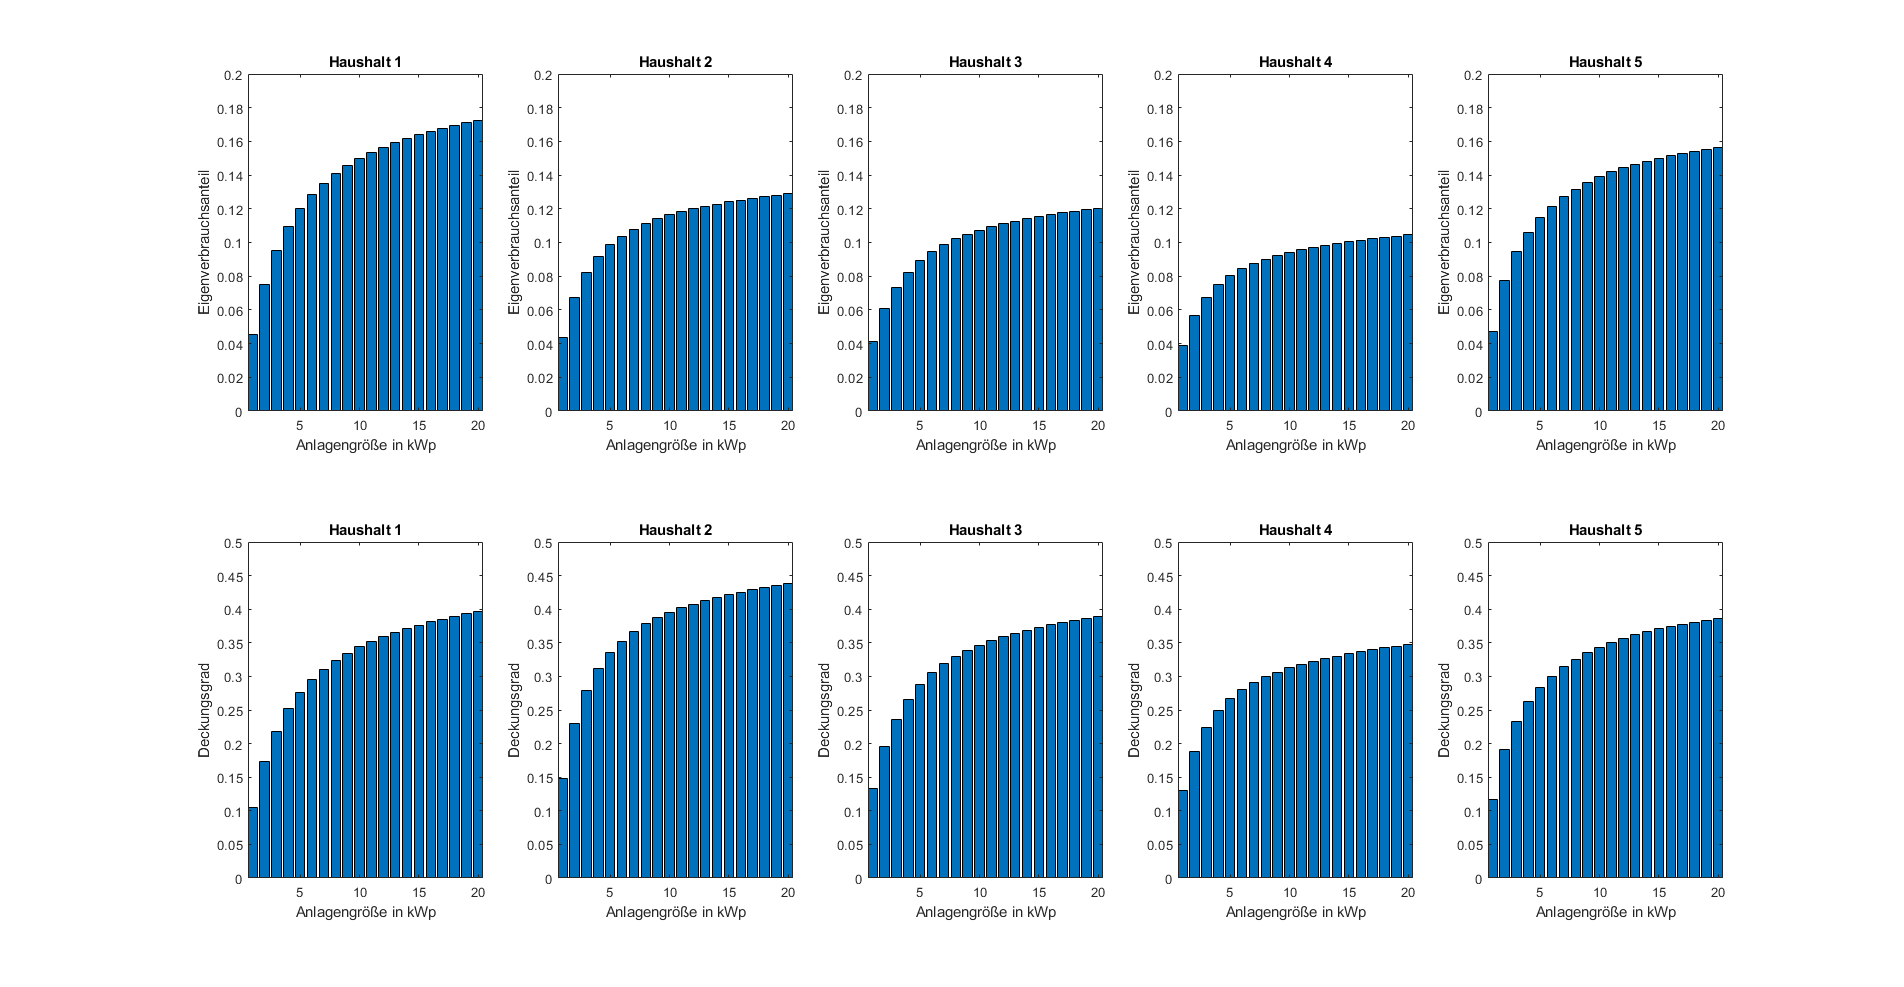
\includegraphics[width=12cm]{img/results/EigenverbrauchDeckungsanteil}
		\caption{Die Entwicklung des Eigenverbrauchsanteils und der Deckungsgrade, der ersten fünf Haushalte, für eine Anlagengröße von $0$ bis $20kWp$.}
	\end{figure}
	\subsubsection{Aufgabe 3.2.c - Darstellung der Last und des Eigenverbrauchs}
	In Aufgabe 3.2.c sollen die Erzeugung, die Last und der Eigenverbrauch für Haushalt 1, in einem Diagramm dargestellt werden.\newline
	Da die Berechnunen hierfür bereits in den Aufgaben 3.2.a durchgeführt wurden, müssen die Daten lediglich noch in dem geforderten $area$ Plot dargestellt werden.\\ \par
	\noindent Der MATLAB Code dazu sieht wie folgt aus:
	\begin{lstlisting}
	Woche_3(:,1)=EigenverbrauchHaushalt_a(1345:2017,1);
	Woche_3(:,2)=LeistungHaushalte(1345:2017,1);
	Woche_3(:,3)=PV_Einspeiseenergie_a(1345:2017);
	
	Woche_25(:,1)=EigenverbrauchHaushalt_a(16129:16801,1);
	Woche_25(:,2)=LeistungHaushalte(16129:16801,1);
	Woche_25(:,3)=PV_Einspeiseenergie_a(16129:16801);
	\end{lstlisting}
	Das daraus resultierende Diagramm wird in Abbildung 3 dargestellt.
	\begin{figure}[H]
		\centering
		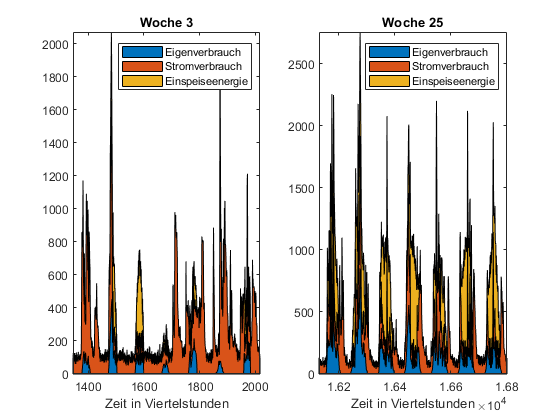
\includegraphics[width=12cm]{img/results/LastundEigenverbrauch}
		\caption{Die Anteile "Eigenverbrauch", "Stromverbrauch" und "Einspeiseenergie" für den Haushalt 1, in den Wochen 3 und 25 des Jahres 2016.}
	\end{figure}
	\noindent Durch die kürzeren Tage in der Woche 3 steigt der Stromverbrauch des Haushaltes, da Energiekonsumenten wie die Beleuchtung und die Beheizung eine längere Zeit aktiv sind. Gleichzeitig sinkt jedoch die Energieproduktion der PV-Anlage aufgrund der geringeren Einstrahlung. Daraus resultiert für die Woche 3 eine sehr geringe Einspeiseenergie.\\ \par
	\noindent In der Woche 25 sinkt der Energiekonsum von Verbrauchern wie der Beleuchtung und der Beheizung, was zu einem wesentlich geringeren Stromverbrauch des Haushaltes beiträgt. Gleichzeitig ist die Einstrahlung in den Sommer-Monaten wesentlich höher, wodurch die Produktion der PV-Anlage steigt. Dadurch resultiert eine Einspeiseenergie für den Haushalt 1.
	\subsection{Aufgabe 3.3}
	\subsubsection{Aufgabe 3.3.a - Vergleich des Barwerts der Haushalte mit und ohne PV-Anlage}
	In Aufgabe 3.3 soll die Investitionsrechnung für die fünf Haushalte aus Aufgabe 3.2 durchgeführt werden. Es wird wieder von einer PV-Anlage mit einer Größe von $5kWp$ ausgegangen.\newline
	Es soll für die Haushalte der Barwert für den Fall mit PV-Anlage mit dem Fall ohne PV-Anlage vergleichen werden. Der Betrachtungszeitraum ist wieder $25$ Jahre.\\ \par
	\noindent Folgender MATLAB Code errechnet sowohl den Barwert für den Fall mit PV-Anlage als auch für den Fall ohne PV-Anlage.
	\begin{lstlisting}
	NPV_mitPV=zeros(1,5);
	NPV_ohnePV=zeros(1,5);
	
	Investitionszuschuss=min(Systemkosten*Anlagenleistung*Investitionszuschuss_prozent, Investitionszuschuss_max*Anlagenleistung_5_2);
	
	for i = 1:5
		NPV_mitPV(i) =$-$Systemkosten*Anlagenleistung_5_2;
		NPV_ohnePV(i) = 0;

		for j = 1:25
			CF_mitPV=EigenverbrauchHaushaltGesamt_a(i)*Haushaltsstrompreis/100+UeberschussHaushalt_a(i)*Einspeisetarif_5_3/100+Investitionszuschuss$-$(StromverbrauchHaushalt_b(i)$-$EigenverbrauchHaushaltGesamt_a(i))*Haushaltsstrompreis/100$-$Betriebskosten*Anlagenleistung;
			NPV_mitPV(i)=NPV_mitPV(i)+CF_mitPV/(1+Zinssatz)^j;
			
			CF_ohnePV=$-$StromverbrauchHaushalt_b(i)*Haushaltsstrompreis/100;
			NPV_ohnePV(i)=NPV_ohnePV(i) + CF_ohnePV/(1+Zinssatz)^j;
		end
	end
	\end{lstlisting}
	\begin{itemize}
		\item \textbf{CF\_mitPV} entspricht den Cash Flows eines Haushaltes mit PV-Anlage.
		\item \textbf{NPV\_mitPV} ist ein Vektor, der für jeden Haushalt den Barwert, für den Fall mit PV-Anlage, nach i Jahren beinhaltet.
		\item \textbf{CF\_ohnePV} entspricht den Cash Flows eines Haushaltes ohne PV-Anlage.
		\item \textbf{NPV\_ohnePV} ist ein Vektor, der für jeden Haushalt den Barwert, für den Fall ohne PV-Anlage, nach i Jahren beinhaltet.
	\end{itemize}
	Abbildung 4 stellt den Barwert der einzelnen Haushalte, für beide Fälle, dar. Obwohl der Barwert in allen Fällen, mit Ausnahme von einem, negativ ist, ist er für den Fall mit PV-Anlage stets höher als für den Fall ohne PV-Anlage. Demnach verbessert sich die Wirtschaftlichkeit der Haushalte durch die Investition in eine PV-Anlage.\\ \par
	\noindent In Abbildung 5 wird die Differenz der beiden Fälle dargestellt.\newline Besonders hervor zu heben ist der Unterschied im NPV, für Haushalt 1, von circa $150.000\mbox{\euro}$.
	\begin{figure}[H]
		\centering
		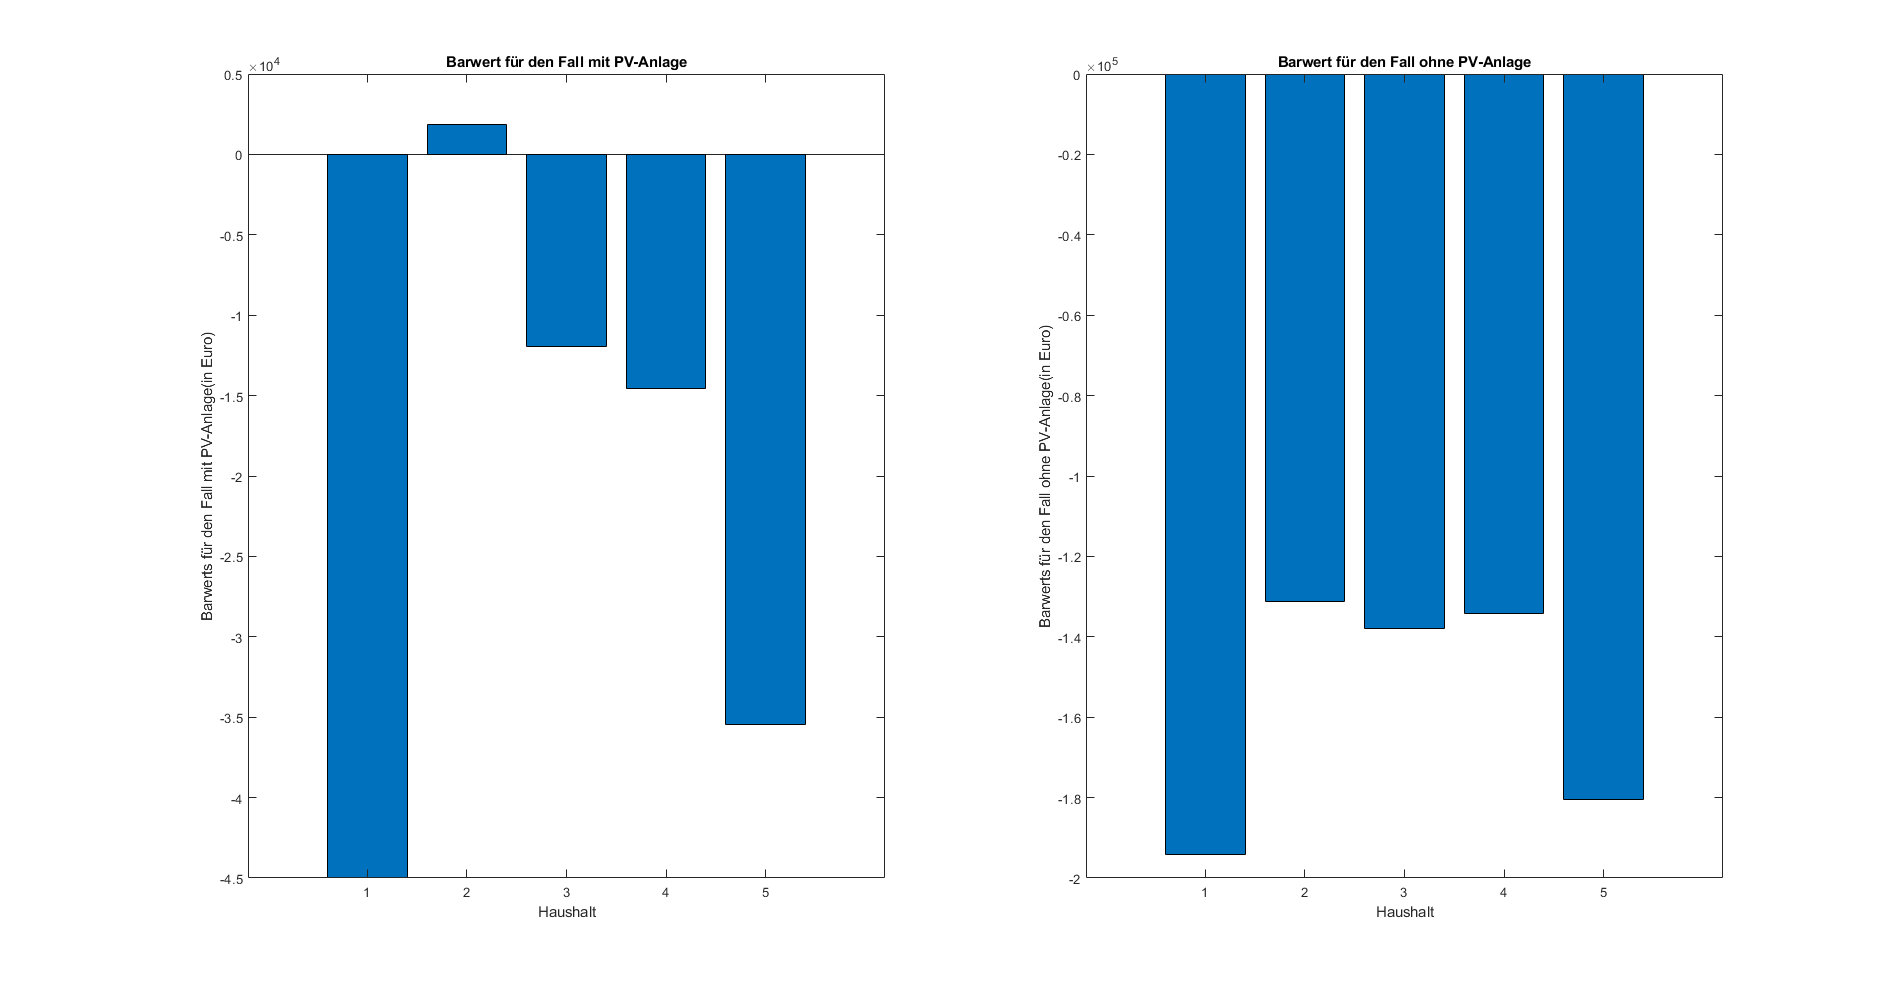
\includegraphics[width=12cm]{img/results/HaushalteBarwerte}
		\caption{Die Barwerte der einzelnen Haushalte, für den Fall mit und ohne PV-Anlage, nach 25 Jahren.}
	\end{figure}
	\begin{figure}[H]
		\centering
		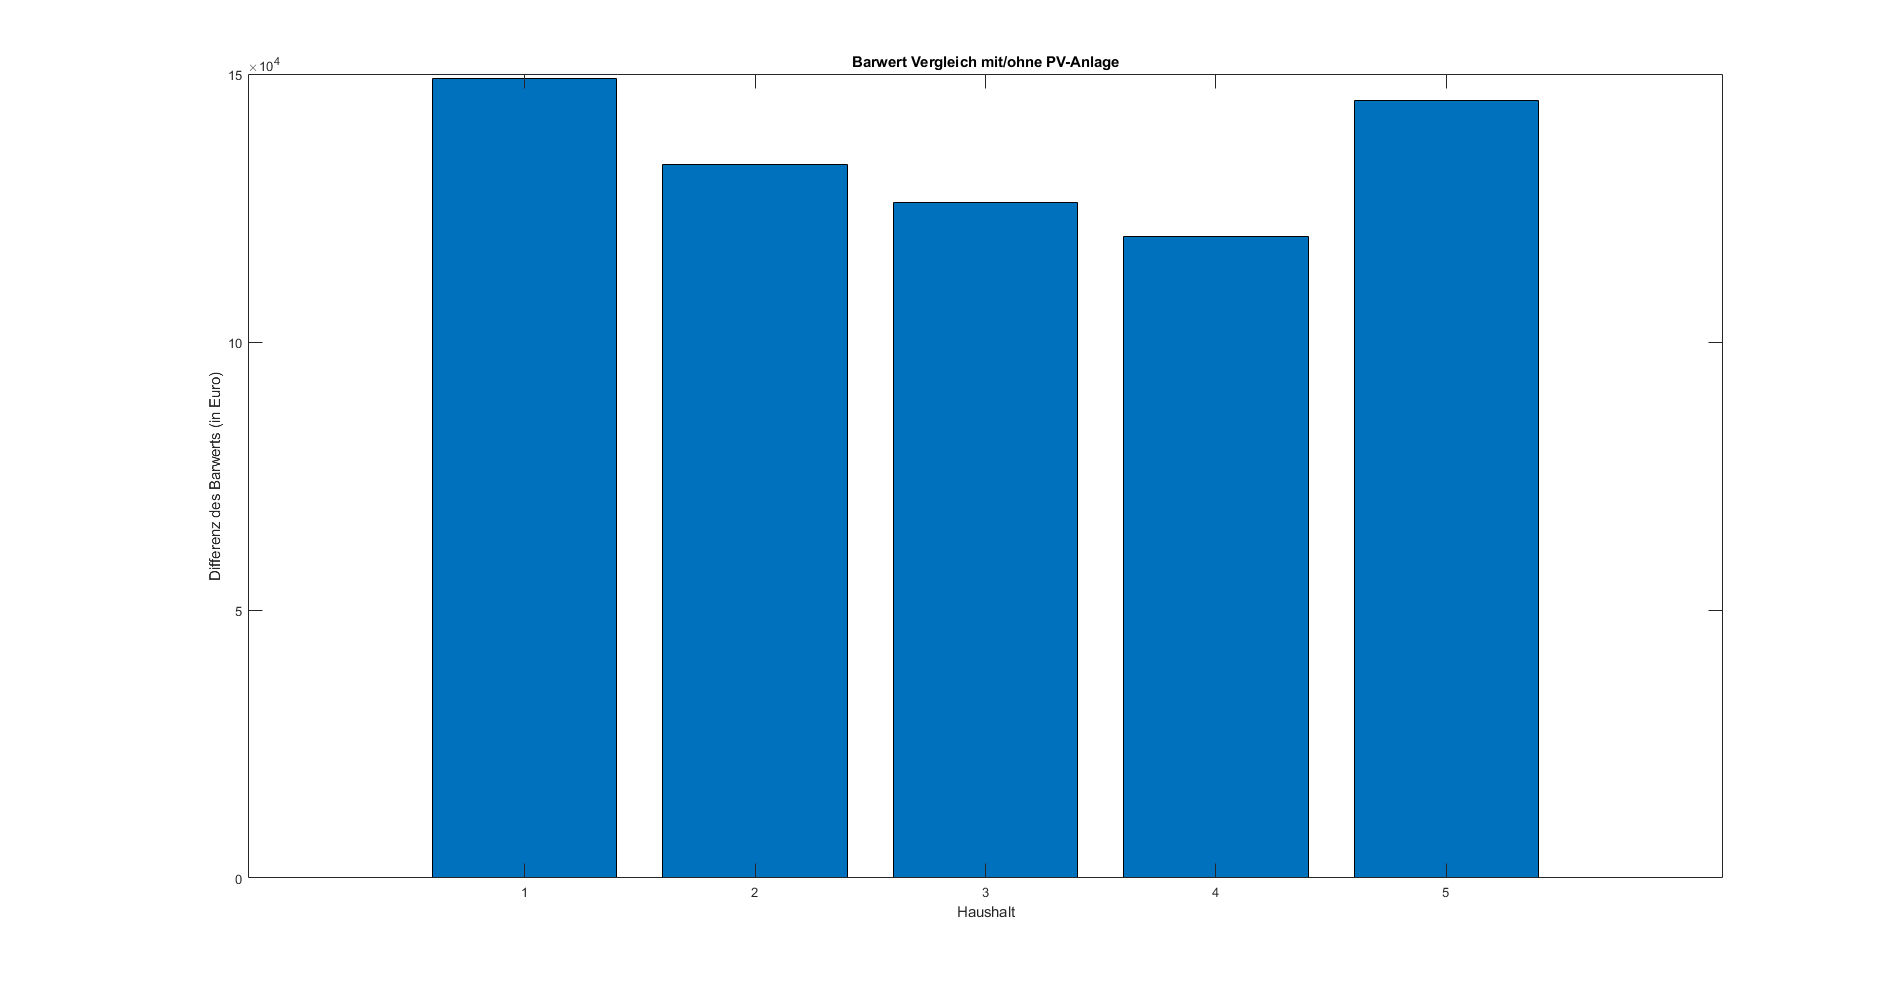
\includegraphics[width=12cm]{img/results/VergleichBarwertMitOhne}
		\caption{Der Unterschied des Barwerts vom Fall mit PV-Anlage, zum Fall ohne PV-Anlage, für jeden Haushalt.}
	\end{figure}
	\subsubsection{Aufgabe 3.3.b - Maximale spezifischen Investitionskosten je Haushalt}
	Für Aufgabe 3.3.b sollen die maximalen spezifischen Investitionskosten je Haushalt errechnet werden.\\ \par
	\noindent Hierzu fügen wir dem MATLAB Code aus Aufgabe 3.3.a folgenden Code hinzu:
	\begin{lstlisting}
	Max_Invest_Vergleich(i)=((NPV_mitPV(i)+Systemkosten*Anlagenleistung_5_2)$-$NPV_ohnePV(i))/Anlagenleistung_5_2;
	\end{lstlisting}
	Die daraus resultierenden maximalen Investitionskosten sind in Tabelle 1 angeführt.
	\begin{table}[H]
		\centering
		\begin{tabular}{|c|c|c|c|c|}
			\hline
			Haushalt 1   & Haushalt 2   & Haushalt 3   & Haushalt 4   & Haushalt 5   \\ \hline
			$3.1030e+04\mbox{\euro}$ & $2.7805e+04\mbox{\euro}$ & $2.6413e+04\mbox{\euro}$ & $2.5125e+04\mbox{\euro}$ & $3.0202e+04\mbox{\euro}$ \\ \hline
		\end{tabular}
	\end{table}
	\subsection{Aufgabe 3.4}
	\subsubsection{Aufgabe 3.4.a - Wirtschaftlichkeit von PV-Anlagen in Österreich}
	\textit{Wie beurteilen Sie auf Basis der in der dieser Übung erlangten Erkenntnisse die Wirtschaftlichkeit von PV-Anlagen in Österreich?}\\ \par
	\noindent Diese Übung hat ergeben, dass der Barwert einer PV-Anlage im Schnitt nach einer Verwendung von nur fünf Jahren positiv wird. Über die gesamte Laufzeit gerechnet ergeben sich durch die Ersparnise bzw. den Verkauf der Überschussleistung beträchtilche Summen. Aus rein elektrischer Sicht ist die Verwendung von PV-Anlagen daher als durchaus wirtschaftlich einzustufen.
	\subsubsection{Aufgabe 3.4.b - Förderung von PV-Anlagen in Österreich}
	\textit{Wie beurteilen Sie auf Basis der in der dieser Übung erlangten Erkenntnisse die Wirtschaftlichkeit von PV-Anlagen in Österreich?}\\ \par
	\noindent Die Förderung von PV-Anlagen ist weiterhin zeitgemäß, weil dadurch auch im privaten Bereich Anreize geschaffen werden. Dies ist notwendig um dem stetig wachsenden Stromverbrauch Herr zu werden.
	\newpage
	\listoffigures
\end{document}